%--------------------------------------------------------------------%
%----------------Monografia de conclusão de curso.-------------------%
%-----------EACH: Escola de Artes Ciências e Humanidades-------------%
%--------------Bacharelado em Sistemas de Informação-----------------%
%----------Discente: Adilson Lopes Khouri N° USP: 6411994------------%
%-----------------Docente: Alexandre Ferreira Ramos------------------%
%--------------------------------------------------------------------%



% Monografia, papel a4, fonte tamanho 10pt.
\documentclass[10pt,a4paper]{report}


% Pacotes e comandos customizados %
% Para digitar e compreender em portugues os comandos
\usepackage[brazil]{babel}
\usepackage[utf8]{inputenc}
\usepackage{indentfirst}
\usepackage[T1]{fontenc}

%Para incluir figuras
\usepackage{graphicx}

%Símbolos matemáticos.
\usepackage{amsmath}
\usepackage{amssymb}
\usepackage{amsthm}

%Permite customizar a legenda das figuras.
\usepackage[small,bf]{caption}

%Define as margens da folha, tamanho...
\usepackage[lmargin=2cm,tmargin=2cm,bmargin=2cm,rmargin=2cm]{geometry}


%Put abntex package


% To type URL with linebreak at special characters.
\usepackage{url}

% Improved and customizable hyphenation patterns.
%\usepackage{hyphenat}
%\hyphenation{pe-rio-do res-pon-sá-vel}

% Pacote de cores
\usepackage{color}
\usepackage{xcolor}        

%Permite a inclusão de código fonte de forma bonita.
\usepackage{listings}
\lstset{		
	language = C, 				% Linguagem de programação
	keywordstyle = \color{blue}, 		% Estilo das palavras chaves
	commentstyle = \color{dkgreen}, 	% Estilo dos Comentários
	stringstyle =  \color{orange}, 		% Estilo de Strings
	numbers=left,
        stepnumber=1,
        firstnumber=1,
        numberstyle=\tiny,
        extendedchars=true,
        breaklines=true,
        frame=tb,
        basicstyle=\footnotesize,
        stringstyle=\color{red},
        showstringspaces=false,
        otherkeywords={FILE, NULL, free, malloc, cos, sqrt, log}
        }
\renewcommand{\lstlistingname}{Código}
\renewcommand{\lstlistlistingname}{Lista de Listagens}


%Permite incluir uma lista do tipo Zebra

%\usepackage{listings}
%\usepackage{xcolor}


%Cria um comando de lista com duas cores de linhas em latex (Estilo 'Zebra').
%\newcommand\realnumberstyle[1]{}

%\makeatletter
%\newcommand{\zebra}[3]{%
 %   {\realnumberstyle{#3}}%
 %   \begingroup
 %   \lst@basicstyle
 %   \ifodd\value{lstnumber}%
 %       \color{#1}%
 %   \else
 %       \color{#2}%
 %   \fi
 %       \rlap{\hspace*{\lst@numbersep}%
 %       \color@block{\linewidth}{\ht\strutbox}{\dp\strutbox}%
 %       }%
 %   \endgroup
%}%
%\makeatother


%% Referências bibliográficas e afins
% Formatar as citações no texto e a lista de referências
\usepackage{natbib}

% Adicionar bibliografia, índice e conteúdo na Tabela de conteúdo
% Não inclui lista de tabelas e figuras no índice
\usepackage[nottoc,notlof,notlot]{tocbibind}


%inserir codigo fonte bonito.
\usepackage{minted}

%\usemintedstyle{borland}
\usemintedstyle{default}
\definecolor{bg_gray}{rgb}{0.95,0.95,0.95}

\renewcommand{\theFancyVerbLine}{
 \sffamily\textcolor[rgb]{0.5,0.5,0.5}{\scriptsize\arabic{FancyVerbLine}}}




\begin{document}

%Esta aqui apenas para n dar erro, deve ser removido.
\cite{Brauman}
\cite{Cprograming}
\cite{DAWKINS}
\cite{HIGHAM}
\cite{Xenopus}
\cite{KLOEDEN}
\cite{PODOLSKY}
\cite{SALINAS}
\cite{SAUER}


%--------------------------------------------------------------------%
%---------------------Capítulos da monografia------------------------%
%-----------------Encontram dentro da pasta Secoes-------------------%
%--------------------------------------------------------------------%


%--------------------------------------------------------------------%
%--------------------------Resumo------------------------------------%
%--------------------------------------------------------------------%
% Mandatory (4.1.9 Resumo na língua vernácula).
\chapter*{Resumo}
%\begin{resumo}

No presente trabalho analisamos o comportamento assimptótico de uma equação diferencial estocástica cuja componente determinística apresenta bi-estabilidade.
O termo determinístico puro é integrável e sua solução é apresentada nesse trabalho. Escolhemos uma condição em que a distância entre as duas soluções assimptóticas estáveis são equidistantes à solução instável.

À equação diferencial ordinária original, introduzimos ruído nos moldes de Langevin, ou seja, pela adição de uma 
"força aleatória", transformando o sistema inicial numa equação diferencial estocástica.
A solução da equação diferencial estocástica é obtida numericamente pelo método de Euler-Maruyama, introduzimos o ruído pelo método de Langevin, adicionando uma força aleatória à equação diferencial ordinária biestável. 
A amplitude da perturbação \textit{($\sigma$)} é um parâmetro livre do nosso sistema e possui três condições distintas.
Pequenos valores de $\sigma$ garantem que a solução somente flutue em torno do limite assimptótico estável correspondente á condição inicial da equação. Por outro lado, para grandes valores de $\sigma$ , a solução flutua em torno do limite assimptótico instável. Por fim, em caso de valores intermediários da amplitude de flutuação, notamos que a solução, para grandes valores de tempo e independente da condição inicial, alterna flutuações aleatórias em torno de uma ou outra das soluções assimptóticas 
estáveis.

Nosso modelo pode ser aplicado para o estudo de sistemas biológicos associados ao desenvolvimento celular. Em geral, uma certa função celular é tratada como uma região de estabilidade. No entanto, sistemas celulares apresentam ruído.
Um exemplo de sistema que apresenta multi-estabilidade são as células de metazoários em que células se especializam em realizar funções específicas dentro do organismo. Podemos associar, a cada possível função celular, uma etiqueta que, em terminologia matemática, podemos chamar de ponto estável.

Se escrevermos uma EDO multi-estável cuja variável dependente é utilizada como etiqueta celular, cada um de seus limites assimptóticos representa uma de suas possíveis funções.
 
 
 
%
%equações diferenciais estocásticas. Solucionamos por meio analitico e numérico (algoritmo de Euler) uma 
%equação diferencial ordinária (que origina a equação diferencial estocástica).
%
%Utilizando o algoritmo de Euler obtivemos resultados da equação diferencial ordinária, 
%plotamos e analisamos os gráficos compreendendo o comportamento da equação em tempos infinitos.
%Após compreender o comportamento do termo determinístico da equação diferencial estocástica adicionamos
%um ruído na mesma obtendo dessa forma a equação diferencial estocástica.
%
%Para solucionarmos a equação diferencial estocástica aplicamos o algoritmo de Euler Maruyama, 
%dessa forma, conseguimos obter resultados sobre seu comportamento em tempos infinitos. 
%
%Por fim comparamos o comportamento das equações: ordinária e estocástica e constatamos que ocorre uma migração de regimes assimptóticos em determinados intervalos de tempo para amplitudes de ruído suficientemente grandes.

%\end{resumo}
%--------------------------------------------------------------------%
%--------------------Término do Resumo-------------------------------%
%--------------------------------------------------------------------%


%--------------------------------------------------------------------%
%------------------------Introdução----------------------------------%
%--------------------------------------------------------------------%
\chapter*{Introdução}

Sistemas celulares apresentam um comportamento que se altera no tempo, um exemplo é o 
processo de determinação do destino celular durante o desenvolvimento de metazoários (FERREL;MACHDLER, 2007).
Uma possível ferramenta matemática para estudar esse tipo de sistema são as 
equações diferenciais ordinárias (EDO's).
Uma EDO relaciona uma função e suas derivadas em relação a variável independente. Uma EDO:
\begin{eqnarray} \label{EDOFormaGeral}
F(t, y^{1}, y^{2},... y^{n}) = 0
\end{eqnarray}
é dita linear se \textit{F} é uma função linear das variáveis: $y^{1}, y^{2},... y^{n}$ em que $y^{k}$ indica a derivada k-ésima da funcao y em relação a uma variável independente \textit{t}. A forma geral de uma EDO linear de ordem \textit{n} pode ser visualizada abaixo:
\begin{equation} \label{LINEAR}
a_{n}(t)y^{(n)}(t) + a_{n-1}(t)y^{(n-1)}(t) +...+ a_{0}(t)y^{(0)}(t) = g(t),
\end{equation}
uma equação que não pode ser escrita na forma (\ref{LINEAR}) é dita não linear segundo BOYCE e DIPRIMA (2000).

Eventualmente, o sistema descrito por uma EDO, pode sofrer 
perturbações aleatórias. 
Por exemplo, o número de constituintes moleculares de uma célula pode flutuar em torno de uma média, 
gerando heterogeneidade em populações celulares. As EDO's apropriadas para esse tipo de fenômeno 
podem ser adidas de um termo de ruído. Nesse caso, elas são chamadas de equações diferenciais estocásticas (EDE's).

EDE's descrevem o comportamento de uma variável aleatória como função do tempo e/ou espaço.
Esta variável satisfaz uma distribuição de probabilidades. Se a distribuição de probabilidades depende do tempo, diremos que o sistema está fora do equilíbrio e, caso contrário, em regime estacionário. Nesta monografia, visamos analisar o comportamento
no equilíbrio de uma EDE cuja componente determinística apresenta bi-estabilidade. 

Um exemplo simples de sistema físico descritível por EDE's são os movimentos do tipo Browniano. Uma partícula realiza deslocamentos sujeitos a interações aleatórias com seu meio. Essas colisões ocorrem a intervalos de tempo e intensidades de força aleatórias. O comprimento dos deslocamentos entre duas colisões (para um número total de colisões macroscópicamente grande \textit{e.g.} $10^{23}$). A variância na posição da partícula cresce com o tempo e indica que a partícula, independentemnte de sua posição inicial, apresentará probabilidades quase idênticas de estar em qualquer posição da superfície do líquido (SILVA;LIMA, 2007).

Por outro lado, em sistemas multi-estáveis, a condição inicial do objeto descrito pela EDO determina seu comportamento para grandes intervalos de tempo. Esses sistemas, quando possuem termos aleatórios, podem apresentar migração entre regimes assimptóticos correspondentes às condições iniciais variadas. Neste projeto, investigaremos quais as formas de ruído que geram esse efeito.

Para proceder com a investigação acima, consideramos a seguinte EDO (em que \textit{a} é uma constante):
\begin{equation} \label{IntroducaoEDO}
\frac{dx}{dt} = -2x(x-a)(x+a) ,
\end{equation}
e a seguinte EDE (EDO acrescida do ruído):
\begin{equation} \label{IntroducaoEDE}
{dx} = -2x(x-a)(x+a)dt + \sigma N(0,1) \sqrt{dt} ,
\end{equation}

Em nosso projeto solucionamos a EDO (\ref{IntroducaoEDO}) numérica e analiticamente e a EDE \newline
(\ref{IntroducaoEDE}) numéricamente através do algoritmo de Euler Maruyama. As soluções numéricas da equação (\ref{IntroducaoEDE}) foram analisadas graficamente e, desta forma, pudemos verificar a migração da solução em torno de cada um dos limites assimptóticos da equação (\ref{IntroducaoEDO}). 

A monografia está estruturada com os seguintes capítulos: ``Modelo Determinístico" onde serão abordados \newline
a EDO, sua solução analítica e sua solução numérica, ``Modelo Estocástico" nesse capítulo será introduzido um ruído na EDO obtendo a EDE a ser analisada e tambem será apresentada a solução numérica da EDE , ``Resultados e Discussão" aqui serão exibidos os gráficos que foram plotados com os resultados de nossa análise da EDO e EDE , ``Aspectos numéricos" onde serão analisados mais a fundo os códigos implementados , ``Conclusão" , ``Referências Bibliografia" e um apêndice com os códigos fonte implementados e um apêndice com Distribuições de variáveis aleatórias e Movimento Browniano.
%--------------------------------------------------------------------%
%--------------------Término da Introdução---------------------------%
%--------------------------------------------------------------------%


%--------------------------------------------------------------------%
%-----------------Distribuições e Mov Browniano----------------------%
%--------------------------------------------------------------------%
\chapter*{Distribuições de variáveis aleatórias e Movimento Browniano}
Serão descritos os algoritmos implementados, seus resultados em forma gráfica e algumas observações que conseguimos obter baseados na análise dos gráficos. Entre essas observações podemos citar: relação entre aumento do número de barras e pontos nos intervalos das variáveis aleatórias, mudanças na semente aleatória e na quantidade de pontos do movimento Browniano. Implementamos em C um algoritmo que gera números pseudo-aleatórios %(\ref{GeradorPseudoAleatoriosFONTE}), este algoritmo é um gerador multiplicativo pois o termo de soma na fórmula é zero. 

Implementamos em C um algoritmo %(\ref{d_Uniforme}) que satisfaz a distribuição uniforme, cuja Função densidade probabilidade (FDP) é dada por:
\begin{equation}
Fdp(X) = \frac{1}{|b-a|}
\end{equation}
\begin{figure}[!htb]
\centering
\begin{minipage}[b]{0.9\linewidth}
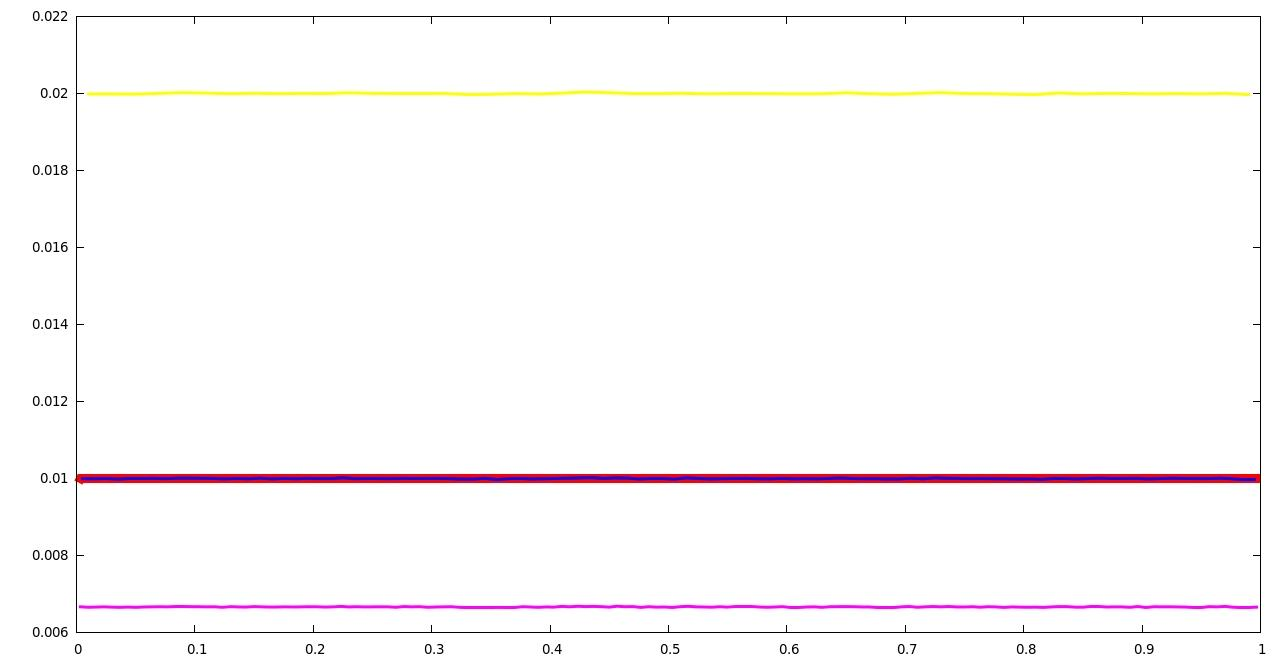
\includegraphics[width=\linewidth]{./img/Distribuicoes/uniVarNumBar.jpg}
\caption{Variação no número de barras da distribuição uniforme.}
\label{figUniformeBar}
\end{minipage} \hfill
\end{figure}
\begin{figure}[!htb]
\centering
\begin{minipage}[b]{0.9\linewidth}
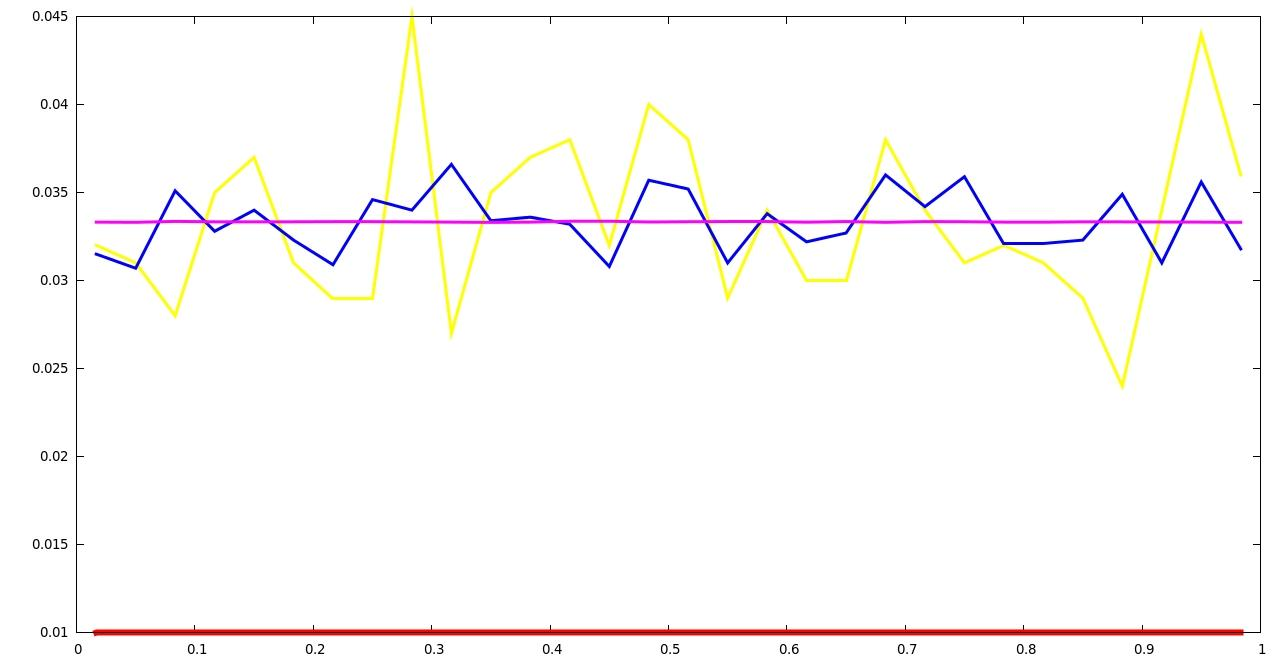
\includegraphics[width=\linewidth]{./img/Distribuicoes/uniVarNumPts.jpg}
\caption{Variação no número de pontos da distribuição uniforme.}
\label{figUniformePt}
\end{minipage} \hfill
\end{figure}


As curvas: vermelha e preta nas figuras (\ref{figUniformeBar}) e (\ref{figUniformePt}) representam variáveis aleatórias satisfazendo uma distribuição uniforme exata. Para plotar essas curvas foi utilizada a probabilidade da variável aleatória assumir um valor qualquer em um intervalo, tal probabilidade é dada pela frequência relativa:
\begin{equation}
f(x) = 0.01.
\end{equation}
Após analisar a figura (\ref{figUniformeBar}), constatamos que a diminuição do número de barras faz a distribuição uniforme se deslocar em direção oposta ao eixo X, já o aumento do número de barras  faz a curva se deslocar em direção ao eixo X. Pode-se verificar essa asserção comparando as curvas: vermelha (ideal), amarelo (50 barras) e rosa (150 barras).

Após análisar a figura (\ref{figUniformePt}) observamos que a acurácia das curvas aumenta ou diminuí (em relação a curva vermelha) de acordo com o aumento ou redução do número de pontos utilizados para plotar as curvas. Para verificar esta asserção pode-se comparar as curvas: amarela (1000pts), azul escuro (10000pts) e rosa ($10^{8} pts$), observa-se que a curva rosa (que possuí maior acurácia e número de pontos que a outras) possuí um comportamento mais próximo da curva vermelha (ideal).

Implementamos em C um algoritmo %(\ref{d_Exponencial}) que satisfaz a distribuição exponencial, ondeé a média , cuja FDP  é:
\begin{equation}
Fdp(X) = \lambda e^{-\lambda x}.
\end{equation}

\begin{figure}[!htb]
\centering
\begin{minipage}[b]{0.9\linewidth}
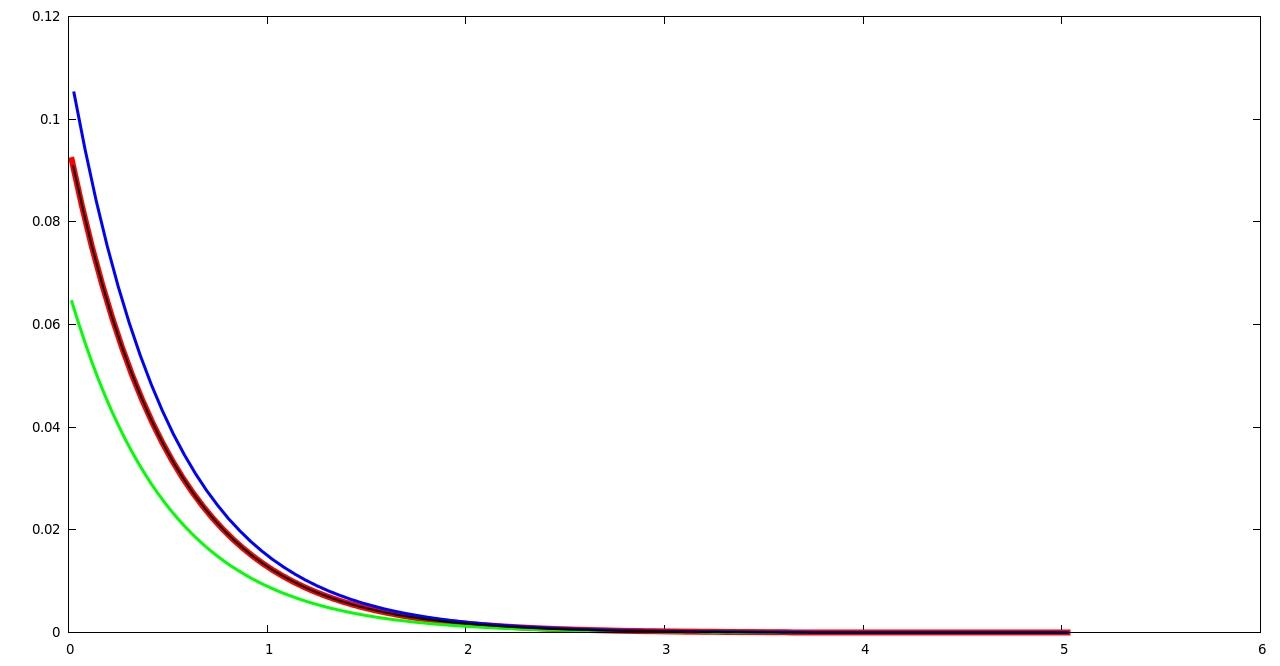
\includegraphics[width=\linewidth]{./img/Distribuicoes/expVarBarr.jpg}
\caption{Variação no número de barras da distribuição exponencial.}
\label{figExpBar}
\end{minipage} \hfill
\end{figure}

\begin{figure}[!htb]
\centering
\begin{minipage}[b]{0.9\linewidth}
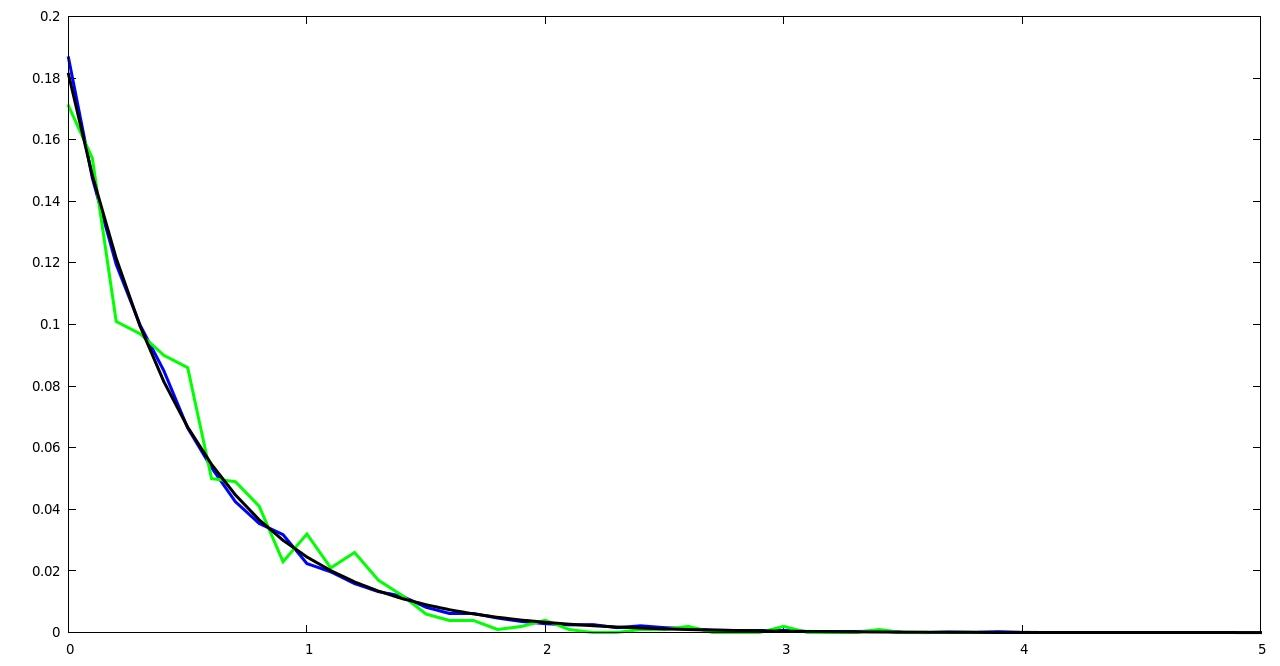
\includegraphics[width=\linewidth]{./img/Distribuicoes/expVarpt.jpg}
\caption{Variação no número de pontos da distribuição exponencial.}
\label{figExpPt}
\end{minipage} \hfill
\end{figure}


As curvas: vermelha e preta das figuras (\ref{figExpBar}) e (\ref{figExpPt}) representam variáveis aleatórias satisfazendo uma distribuição exponencial exata. Para plotar essas curvas foi utilizada a probabilidade da variável aleatória assumir um valor qualquer em um intervalo, tal probabilidade é dada pela frequência relativa:
\begin{equation}
f(X) = e^{-2x} - e^{-2(x+ 0.05)}.
\end{equation}

Após analisar a figura (\ref{figExpBar}), constatamos que a diminuição do número de barras faz a distribuição exponencial se deslocar em direção ao eixo X, já o aumento do número de barras  faz a curva se deslocar em direção contrária ao eixo X. Pode-se verificar essa asserção comparando as curvas: vermelha (ideal), verde (90 barras) e azul escuro (150 barras). 

Após análisar a figura (\ref{figExpPt}) observamos que a acurácia das curvas aumenta ou diminuí (em relação a curva preta) de acordo com o aumento ou redução do número de pontos utilizados para plotar as curvas. Para verificar esta asserção pode-se comparar as curvas: verde (1000pts), azul escuro (10000pts) e preto ($10^{8}pts$), observa-se que a curva azul (que possuí maior acurácia e número de pontos que a verde) possuí um comportamento mais próximo da curva rosa (ideal).

Codificamos em C  um algoritmo %(\ref{d_Gaussiana}) que gera uma variável aleatória que satisfaz uma Gaussiana normal de média 0 e variância 1 (N(0,1)) e  cuja FDP é:
\begin{equation}
FDP = \frac{1}{ \sigma  \sqrt{2 \pi } } e^{ \frac{-(x - \mu )^{2}}{{2 \sigma ^{2}}}}
\end{equation}
A variável aleatória satisfazendo uma distribuição Gaussiana com média 0 e variância 1, é de importância crucial para nosso trabalho. O movimento Browniano utiliza uma Gaussiana para gerar seus pontos e o algoritmo de Euler Maruyama utiliza o movimento Browniano para solucionar o termo estocástico da equação %(\ref{Cubo}).

\begin{figure}[!htb]
\centering
\begin{minipage}[b]{0.9\linewidth}
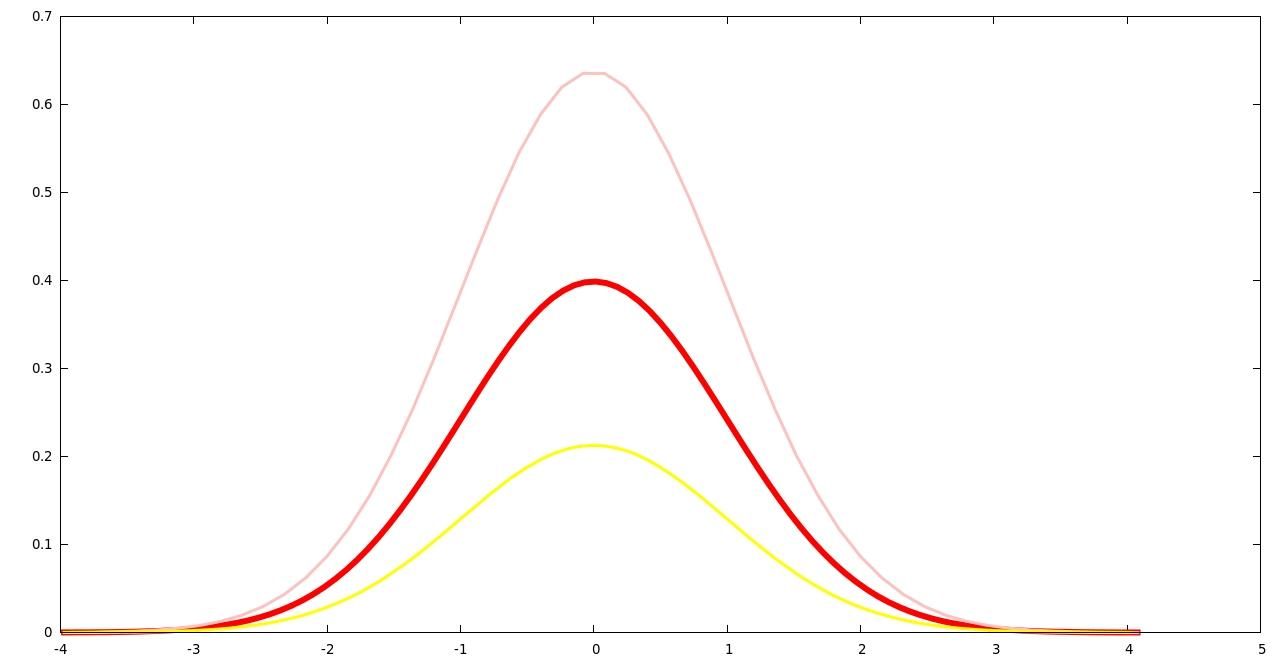
\includegraphics[width=\linewidth]{./img/Distribuicoes/GauVarBar.jpg}
\caption{Variação no número de barras da distribuição Gaussiana.}
\label{figGaussianaBar}
\end{minipage} \hfill
\end{figure}

\begin{figure}[!htb]
\centering
\begin{minipage}[b]{0.9\linewidth}
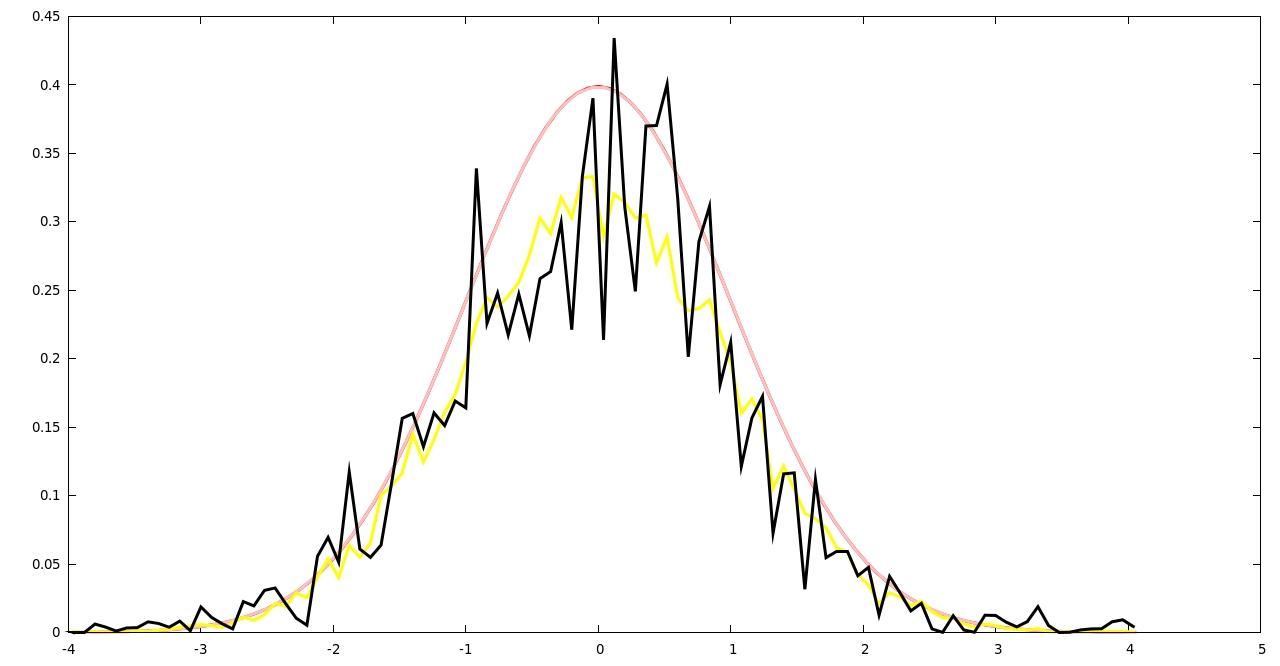
\includegraphics[width=\linewidth]{./img/Distribuicoes/GauVarPt.jpg}
\caption{Variação no número de pontos da distribuição Gaussiana.}
\label{figGaussianaPt}
\end{minipage} \hfill
\end{figure}

Obs.: As curvas vermelha e rosa das figuras (\ref{figGaussianaBar}) e (\ref{figGaussianaPt}) representam uma distribuição Gaussiana exata. Para plotar essas curvas foi utilizada a probabilidade da variável aleatória assumir um valor qualquer em um intervalo, tal probabilidade é dada pela frequência relativa da Gaussiana
\begin{eqnarray}
f(x) = \frac{1}{\sqrt{2 \pi}}exp(-\frac{x^{2}}{2})
\end{eqnarray}
Após analisar a figura (\ref{figGaussianaBar}) constatamos que a redução do número de barras faz a distribuição Gaussiana se deslocar em direção ao eixo X, um aumento do número de barras a desloca no sentido contrário ao eixo X. Essa constatação pode ser observada comparando as curvas vermelha (ideal), amarela (90 barras) e curva rosa (150 barras).
 
Atráves da figura (\ref{figGaussianaPt}) observamos que a acurácia das curvas aumenta ou diminuí (em relação a curva rosa) de acordo com o aumento ou redução do número de pontos utilizados para plotar as curvas. Para verificar esta asserção pode-se comparar as curvas: preta (1000pts), amarela (10000pts) e rosa ($10^{8}pts$), observa-se que a curva amarela (que possuí maior acurácia e número de pontos que a preta) possuí um comportamento mais próximo da curva rosa (ideal).	
\begin{figure}[!htb]
\centering
\begin{minipage}[b]{0.9\linewidth}
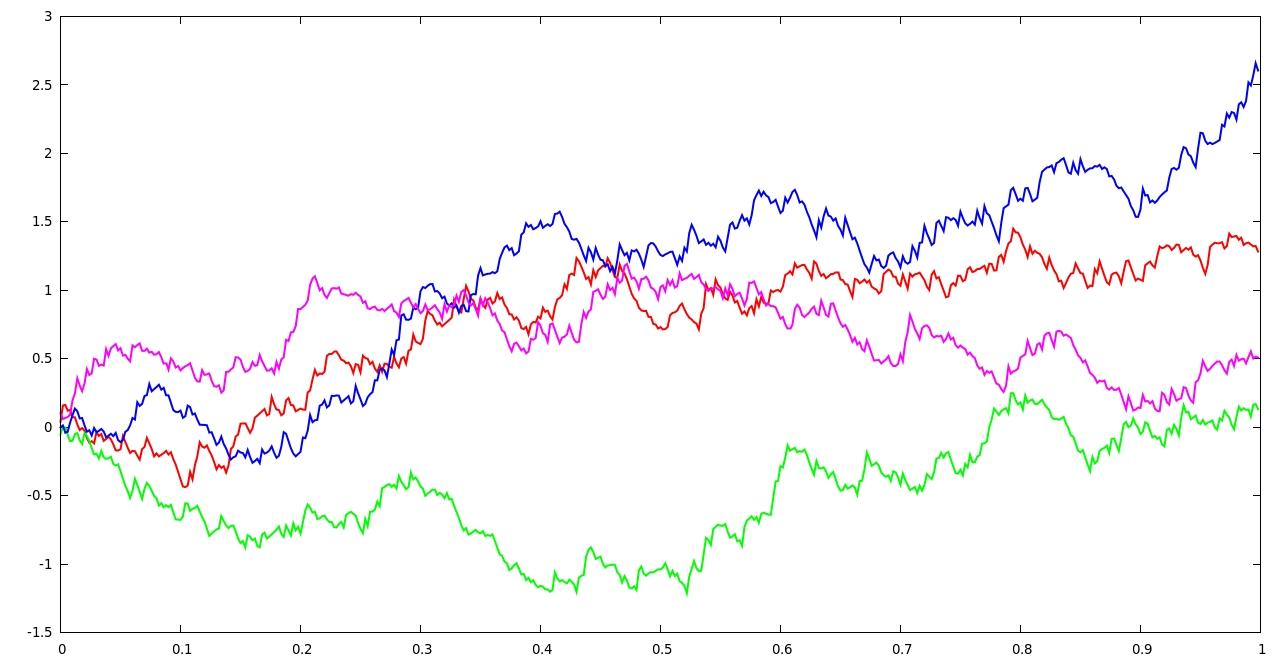
\includegraphics[width=\linewidth]{./img/Distribuicoes/Mb500pts.jpg}
\caption{Movimento Browniano com 500 pontos.}
\label{figMovBrown500}
\end{minipage} \hfill
\end{figure}

\begin{figure}[!htb]
\centering
\begin{minipage}[b]{0.9\linewidth}
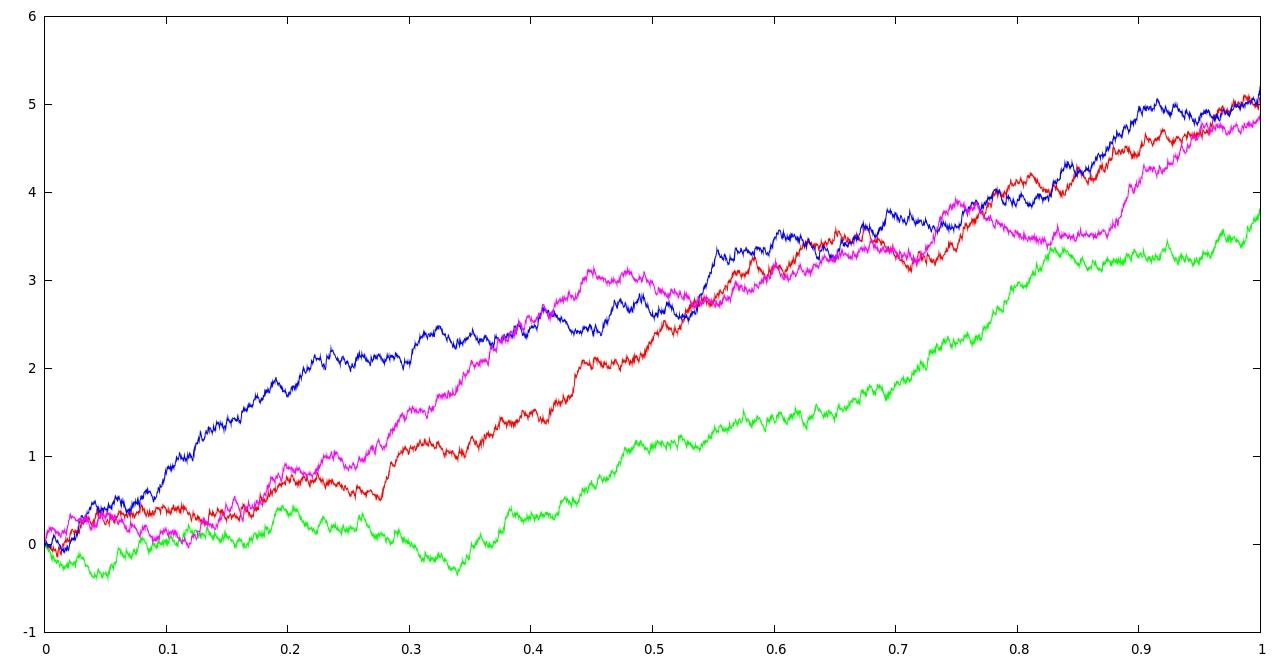
\includegraphics[width=\linewidth]{./img/Distribuicoes/MB5000ptos.jpg}
\caption{Movimento Browniano com 5000 pontos.}
\label{figMovBrown5000}
\end{minipage} \hfill
\end{figure}
Implementamos em C um algoritmo que gera o movimento Browniano %(\ref{movimentoBrownianoFONTE}) que utiliza uma variável aleatória Gaussiana de média 0 e variância 1 (N(0,1)). As figuras (\ref{figMovBrown500}) e (\ref{figMovBrown5000}) representam execuções do algoritmo que gera o movimento Browniano, as seguintes sementes aleatórias foram escolhidas: 34, 67, 157, 229. No caso da figura (\ref{figMovBrown500}), foram utilizados 500 pontos, a figura (\ref{figMovBrown5000}) utilizou 5000 pontos.
%--------------------------------------------------------------------%
%---------------Término da distribuições e Mov Browniano-------------%
%--------------------------------------------------------------------%


%--------------------------------------------------------------------%
%-------------------Modelo deterministico----------------------------%
%--------------------------------------------------------------------%
\chapter{Modelo determinístico}
Este capítulo é devotado a análise do regime estacionário, a solução analítica e numérica da seguinte equação:
\begin{eqnarray}\label{ModeloDeterministicoEDO}
\frac{dx}{dt} = -2x(x-a)(x+a) ,
\end{eqnarray}
em que \textit{x} é função do tempo, \textit{t} é a variável independente e 
\textit{a} é uma constante arbitrária real positiva da equação.

\section{Análise do regime estacionário} 
Nesta seção, analisamos o regime estacionário que será assumido pela equação (\ref{ModeloDeterministicoEDO}). O regime estacionário ocorre sob a condição:
\begin{eqnarray}\label{eq1}
\frac{dx}{dt} = 0.
\end{eqnarray}
Nesse caso, queremos verificar a existência de pontos de equilíbrio, bem como classificá-los como estáveis ou instáveis.
A equação (\ref{ModeloDeterministicoEDO}) apresenta três pontos de equilíbrio, para os valores assimptóticos de \textit{x} dados por:
\begin{eqnarray}
\overline{x}_{\pm} &=& \pm a , \\
\overline{x}_{0} &=& 0 ,
\end{eqnarray}
que são obtidos a partir do cálculo das raízes do polinômio de grau três:
\begin{eqnarray}\label{eq111}
-2 \overline{x}(\overline{x} - a)(\overline{x} + a) = 0.
\end{eqnarray}
Para classificarmos os pontos $\overline{x}_{\pm}$ , $\overline{x}_{0}$ em estáveis ou instáveis, podemos considerar somente o lado direito da equação (\ref{ModeloDeterministicoEDO}):
\begin{eqnarray}
s(x) = -2 \overline{x}(\overline{x} - a)(\overline{x} + a) = 0.
\end{eqnarray}
Essa equação possui raízes $\overline{x}_{\pm}$ , $\overline{x}_{0}$, e seu gráfico é da forma:
\begin{figure}[!htb]
\centering
\begin{minipage}[b]{0.55\linewidth}
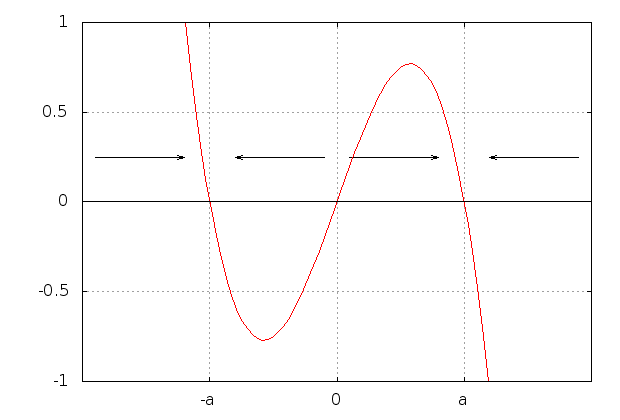
\includegraphics[width=\linewidth]{./img/secao2_1/camposDirecao.png}
\caption{Pontos de equilíbrio.}
\label{camposDirecao}
\end{minipage} \hfill
\end{figure}
e pode ser interpretado como segue. O valor de $\frac{dx}{dt}$, será positivo e causará incremento em $x(t)$ nos casos:
\begin{itemize}
\item[i)] x(t) < -a;
\item[ii)] 0 < x(t) < a.
\end{itemize}
Por outro lado, $x(t)$ decresce sob as condições:
\begin{itemize}
\item[iii)] 0 > x(t) > -a;
\item[iv)] x(t) $>$ a.
\end{itemize}
Assim, se a condição \textit{i} ou \textit{iii} ocorrerem, o sistema tende a alcançar o ponto $x = -a$. Já o ponto $x = a$ é atingido no caso de as condições \textit{ii} ou \textit{iv} ocorrerem. Para a condição \textit{i}, temos $y < 0 $ e $\frac{dy}{dt} > 0 $ e na condição \textit{iii}, $y < 0$ e $\frac{dy}{dt} < 0$. 

As condições \textit{ii} e \textit{iv} indicam respectivamente, $y > 0$ e $\frac{dy}{dt} > 0$ e $y > 0$ e $\frac{dy}{dt} < 0$. A dinâmica de $y(t)$ sob as condições \textit{i}, \textit{ii}, \textit{iii} e \textit{iv} é indicada por flechas horizontais da figura (\ref{camposDirecao}). Note que $\frac{dy}{dt} \rightarrow 0$ nas vizinhanças dos pontos $\overline{x}_{\pm}$ e $\overline{x}_{0}$, indicando que estes são pontos de equilíbrio do sistema.

Um próximo passo consiste em determinar as concavidades das soluções de $x(t)$ da equação (\ref{ModeloDeterministicoEDO}). Para isso, verificamos o sinal da segunda derivada de $x(t)$ em relação a \textit{t}. Assim, aplicando a regra da cadeia:
\begin{eqnarray} \label{regraDaCadeiaDerivadaSegunda}
\frac{d^{2}x}{dt^{2}} = \frac{d}{dt} s(x) = \frac{ds}{dx} \frac{dx}{dt},
\end{eqnarray}
explicitamente obtemos:
\begin{eqnarray}
\frac{d^{2}x}{dt^{2}} = 4x (x-a) (x+a)(\sqrt{3} x-a)(\sqrt{3} x+a),
\end{eqnarray}
e assim, para $x < -a$, $x"(t) < 0$, e a concavidade será para baixo. Se tomarmos $x > a$, temos $x"(t) > 0$ e concavidade para baixo. Se tomarmos $x > a$ ,  $x"(t) > 0$ e a concavidade é para cima, tomando $-a < x < - \frac{a}{\sqrt{3}}$, $x"(t) < 0$ e a concavidade é para baixo. Se tomarmos $-\frac{a}{\sqrt{3}} < x < 0$, $x"(t) < 0$ e a concavidade é para baixo, se tomarmos $0 < x < \frac{a}{\sqrt{3}}$, $x"(t) > 0$ e a concavidade é para cima e por fim se tomarmos $\frac{a}{\sqrt{3}} < x < a$, $x"(t) > 0$ e a concavidade é para cima.


\section{Solução analítica}
Nesta seção, apresentamos a solução analítica da EDO(\ref{ModeloDeterministicoEDO}). Que pode ser escrita em termos de uma condição inicial $x(0) = x_{0}$ como:
\begin{eqnarray}\label{eq134}
x(t) = \pm \frac{a}{\sqrt{(1-(1-\frac{a^{2}}{x_{0}^{2}})e^{-4ta^{2}})}}, |x(0)| > a \\
x(t) = \pm \frac{a}{\sqrt{1+(\frac{a^{2}}{x_{0}^{2}}-1)e^{-4ta^{2}}}} , |x(0)| < a.
\end{eqnarray}
Para calcularmos as soluções acima para a equação (\ref{ModeloDeterministicoEDO}), nós a reescrevemos na forma:
\begin{eqnarray}
\frac{dx}{-2x(x-a)(x+a)} = dt.
\end{eqnarray}
Em seguida devemos integrar ambos os lados da equação como segue:
\begin{eqnarray}
\int_{x(0)}^{x(t)}{\frac{dx}{-2x(x-a)(x+a)}} = \int_{0}^{t}{dt}.
\end{eqnarray}
Para calcularmos a integral à esquerda da igualdade, primeiro decompomos a integral como a seguinte soma:
\begin{eqnarray}\label{Reescrita3Termos}
\int \frac{dx}{-2x(x-a)(x+a)} = \int \frac{A dx}{-2x} + \int \frac{B dx}{(x-a)} + \int \frac{C dx}{(x+a)} , 
\end{eqnarray}
onde A, B e C são constantes definidas em termos de \textit{a}. Os integrais da equação (\ref{Reescrita3Termos}) são da forma $\frac{1}{x}$ e sua solução é da forma $\ln|x| + K$ onde \textit{K} é constante de integração, solucionando a integral do lado direito temos:
\begin{eqnarray}\label{Integrada5}
\frac{1}{2a^{2}} \ln (|x|) + \frac{-1}{4a^{2}} \ln (|x-a|) + \frac{-1}{4a^{2}} \ln (|x+a|) + K \\ ou
\int \frac{dx}{-2x(x-a)(x+a)} = \ln \biggl( \biggl | 1 - \frac{a^{2}}{x^{2}} \biggr | \biggr ) + K.
\end{eqnarray}
Como a função $\ln$ deve ter argumento positivo devemos tratar dois casos: o primeiro onde $|x(0)| > a$ e o segundo onde $|x(0)| < a$. Para o caso onde $|x(0)| > a$ temos como solução:
\begin{eqnarray}\label{Integrada2}
\ln \biggl( \biggl | 1 - \frac{a^{2}}{x^{2}} \biggr | \biggr)^{-\frac{1}{4a^{2}}} + K = t \Leftrightarrow \ln \biggl( \biggl | 1 - \frac{a^{2}}{x^{2}} \biggr | \biggr) = 4a^{2}(-t+K), K  \in \mathbb{R} 
\end{eqnarray}
aplicando a função exponencial em ambos os lados da igualdade e efetuando alguma manipulação algébrica, obtemos:
\begin{eqnarray}\label{Integrada3}
x(t) = \pm \frac{a}{\sqrt{(1- \overline K e^{-4ta^{2}} )}},  t  \in \mathbb{R} ,  t  \in (0, +\infty),
\end{eqnarray}
e, a constante $\overline{K}$ é dada por $e^{4Ka^{2}}$. Podemos definir $\overline{K}$ a partir das condições iniciais do sistema. Assim, para $x(0) = x_{0},$ temos:
\begin{eqnarray}\label{X2}
x_{0} = \pm \frac{a}{\sqrt{1-\overline{K}}} \Leftrightarrow \overline{K} = 1- \frac{a^{2}}{x_{0}^{2}}
\end{eqnarray}
Assim $|x(0)| > a$ , temos:
\begin{eqnarray}\label{S}
x(t) = \pm \frac{a}{\sqrt{1-(1-\frac{a^{2}}{x_{0}^{2}})e^{-4ta^{2}}}}
\end{eqnarray}
Por outro lado, no caso de condições iniciais que satisfaçam: $|x(0)| < a$ temos como solução:
aplicar a função exponencial em ambos os lados da igualdade, obtendo:
\begin{eqnarray}\label{Integrada4}
\ln \biggl( \biggl | \frac{a^{2}}{x^{2}} - 1 \biggr | \biggr)^{-\frac{1}{4a^{2}}} + K = t \Leftrightarrow \ln \biggl( \biggl | \frac{a^{2}}{x^{2}} - 1 \biggr | \biggr) = 4a^{2}(-t+K), 
\end{eqnarray}
aplicando a função exponencial em ambos os lados da igualdade e efetuando alguma manipulação algébrica, obtemos:
\begin{eqnarray}\label{Integrada6}
x(t) = \pm \frac{a}{\sqrt{( -1 + \overline{K} e^{-4ta^{2}} )}},  t  \in \mathbb{R} ,  t  \in (0, +\infty),
\end{eqnarray}
e, a constante $\overline{K}$ é dada por $e^{4Ka^{2}}$. Podemos definir $\overline{K}$ a partir das condições iniciais do sistema. Assim, para $x(0) = x_{0},$ temos:
\begin{eqnarray}\label{X}
x_{0} = \pm \frac{a}{\sqrt{-1+\overline{K}}} \Leftrightarrow \overline{K} = \frac{a^{2}}{x_{0}^{2}} - 1
\end{eqnarray}
Assim para $|x(0)| < a$ , temos:
\begin{eqnarray}\label{S2}
x(t) = \pm \frac{a}{\sqrt{1+(\frac{a^{2}}{x_{0}^{2}} - 1)e^{-4ta^{2}}}}
\end{eqnarray}
Note que, para $x_{0} = \pm a $ , o sistema já se encontra no estado estável e, portanto não há dinâmica. No limite em que $x_{0}$ tende à zero, temos $x(t) \rightarrow 0$ .
O termo positivo da solução é tomado quando o sinal de $x_{0}$ é positivo ou negativo e garante $x(0) = x_{0} $ , independente do sinal, se tomarmos $ \sqrt{x_{0}^{2}} = |x_{0}| = +x_{0}$. No caso de tomarmos $ \sqrt{x_{0}^{2}} = |x_{0}| = -x_{0}$ então a solução negativa é utilizada. 

\section{Solução numérica via método de Euler}
Dada uma equação diferencial ordinária da forma:
\begin{eqnarray}\label{FormaEDO}
\frac{dy}{dt} = f(y),
\end{eqnarray}
cuja solução não seja conhecida, podemos obter valores de $y(t)$ para um intervalo de tempo  $0 \leq t \leq T $, utilizando o método de Euler. O algoritmo para cálculo de solução numérica pode ser escrito como segue:
\begin{eqnarray}\label{AlgoritmoEuler}
y_{n+1} = y_{n} + f_{n} h \hspace{0.7cm} n = 0,1,2...
\end{eqnarray} 
onde $h$ representa um incremento temporal infinitesimal, $f_{n} = f(y_{n})$ , $y_{n} = y(t_{n})$ denota o valor de $y$ no instante $t = nh$ sob a condição inicial $y(t_{0}) = y_{0}$ que é conhecida. O método de Euler consiste em solucionar a equação (\ref{AlgoritmoEuler}) iterativamente utilizando o resultado anterior ($y_{n}$) no cálculo do próximo ($y_{n+1}$), dessa forma são obtidos valores: $y_{0}, y_{1},... y_{n}$ que aproximam a solução $y(t)$ nos pontos: $t_{0}, t_{1}, ... t_{n}$. Substituindo os valores do algoritmo de Euler pelos valores da EDO (\ref{ModeloDeterministicoEDO}):
\begin{eqnarray}
y_{n+1} &\rightarrow & x_{n},    \\
f_{n} &\rightarrow & -2x_{n}(x_{n}-a)(x_{n}+a), 
\end{eqnarray}
obtemos a seguinte relação de recorrência:
\begin{eqnarray}\label{AplicacaoEuler}
x_n = x_{n-1} - 2x_{n-1}(x_{n-1} - a)(x_{n-1} + a)h ,
\end{eqnarray}
que pode ser empregada no estudo numérico da equação (\ref{ModeloDeterministicoEDO}).
%--------------------------------------------------------------------%
%---------------Término do Modelo deterministico---------------------%
%--------------------------------------------------------------------%


%--------------------------------------------------------------------%
%-------------------Modelo Estocástico-------------------------------%
%--------------------------------------------------------------------%
\chapter*{Modelo Estocástico}

Este capítulo é devotado à análise da EDO:
\begin{eqnarray} \label{bola}
\frac{dx}{dt} = -2x(x-a)(x+a) ,
\end{eqnarray}
quando acrescida de uma perturbação aleatória. Há sistemas cuja descrição em termos de EDO é insuficiente. Isto ocorre quando flutuações aleatórias levam a dinâmica a assumir comportamentos muito diferentes da média. Um exemplo é o processo de determinação do destino celular (FERREL;MACHDLER, 2007), em que flutuações da condição ambiental em que a célula está inserida podem levá-la a assumir funções distintas no organismo.
A forma geral de uma EDO acrescida de ruído fica:
\begin{eqnarray}\label{triangulo}
dx = a(x,t)dt + b(x,t) d\xi(t)
\end{eqnarray}
em que a componente $a(x,t)dt$ é herdada do sistema determinístico enquanto a estocasticidade é dada pelo termo $b(x,t)d\xi(t)$. Ao ser acrescida de um fator estocástico $b(x,t)d\xi(t)$ a EDO (\ref{bola}) pode ser denominada EDE (KLOEDER; PLATEN, 1995). O elemento $b(x,t)$ é uma função conhecida enquanto $d\xi(t)$ é um incremento aleatório. A EDE associada é escrita na forma:
\begin{eqnarray}\label{Cubo}
{dx} = -2x(x-a)(x+a)dt + \sigma N(0,1) \sqrt{dt} ,
\end{eqnarray}
em que $x(t)$ é a variável "aleatória" do sistema. Aqui consideramos $b(x,t) = \sigma $ como uma constante que chamamos amplitude de ruído. O termo $N(0,1) \sqrt{dt}$ é o infinitésimo aleatório, em que $N(0,1)$ é um número real que satisfaz uma distribuição normal de média nula e variância um.
Em geral, o ruído incluído na equação (\ref{Cubo}) garante que a dinâmica do valor médio da variável aleatória $x(t)$ na equação (\ref{Cubo}) seja idêntica à dinâmica determinística. Isto pois a média da variável de ruído é nula e não contribui quando tomamos o valor médio da equação (\ref{Cubo}). Conforme verificaremos adiante, esse não será, necessáriamente, o caso. Por sua vez, a variância do incremento aleatório é proporcional à ${\sigma}$ e à $dt$.

\section{Solução Numérica via método de Euler Maruyama}

A equação (\ref{Cubo}) pode ser solucionada numericamente pelo emprego do algoritmo de Euler-Maruyama (KLOEDER; PLATEN, 1995). Assim, dada a EDE  (\ref{triangulo}) e a condição inicial $x(0) = x_0 , $ podemos realizar uma dinâmica da variável $x(t)$ no intervalo  $0 \leq t \leq T$ , através da seguinte relação de recorrência:
\begin{equation}\label{FormaGeralEDE}
X_{n+1} = X_{n} + a(X_{n})dt + b(X_{n})d\xi , \hspace{0.7cm} n = 0,1,2... 
\end{equation}
em que o incremento temporal é indicado por $dt$ e o estocástico por $d\xi$, $a(x,t)dt$ é herdada do sistema determinístico enquanto a estocasticidade é dada pelo termo $b(x,t)d\xi(t)$ e $X_{n} = X(t_{n})$ e $t_{n} = ndt$ que denota o valor de $x$ no instante $\frac{T}{dt}$. O elemento $b(x,t)$ é uma função conhecida enquanto $d\xi(t)$ é um incremento aleatório.A constante \textit{N} é dada como $\frac{T}{dt}$. Para a EDE (\ref{Cubo}), podemos escrever o algoritmo Euler Maruyama. Portanto assumindo as substituições:
\begin{eqnarray}
X_{n} &\rightarrow & x_{n}, \label{teste1}   \\
a(X_{n}) &\rightarrow & -2x_{n}(x_{n}-a)(x_{n}+a), \label{teste2} \\
b(X_{n}) &\rightarrow & {\sigma}, \label{teste3} \\
dt &\rightarrow & h, \label{teste4} \\
d\xi &\rightarrow & N(0,1) \sqrt{h}, \label{teste5} \\
h &\rightarrow & \frac{T}{N}
\end{eqnarray}
relação de recorrência que resolvemos fica:
\begin{eqnarray}\label{EM}
x_{n+1} = x_{n} - 2x_{n}(x_{n} - a)(x_{n} + a)h + \sigma N(0,1) \sqrt{h}
\end{eqnarray}
em que $N(0,1)$ é um número real que satisfaz uma distribuição normal de média nula e variância um. A equação (\ref{EM}) será utilizada para calcular as soluções numéricas da equação (\ref{Cubo}).

%--------------------------------------------------------------------%
%_---------------Término do Modelo Estocástico-----------------------%
%--------------------------------------------------------------------%


%--------------------------------------------------------------------%
%---------------Resultados e Discussão-------------------------------%
%--------------------------------------------------------------------%
\chapter{Resultados e Discussão}
Neste capítulo discutimos os resultados obtidos durante a execução de nosso projeto. Na primeira parte apresentamos os gráficos da solução determinística da equação (\ref{ModeloDeterministicoEDO}). A dinâmica obtida a partir da solução numérica do sistema estocástico, apresentado na equação (\ref{EM}) é apresentada na segunda parte desse capítulo. 

\section{Resultados EDO}
Nessa seção exibimos graficamente, a dinâmica da solução analítica da EDO (\ref{eq1}). Assumimos o parâmetro de etiquetagem igual a uma unidade ($a = 1 $ e $ a = -1$). A solução apresentada na equação (\ref{eq1}) toma a forma:
\begin{eqnarray}\label{eq11111}
x(t) = \pm \frac{a}{\sqrt{(1- (1-\frac{a^{2}}{x_{0}^{2}}) e^{-4ta^{2}})}} , |x(0)| > a \\
x(t) = \pm \frac{a}{\sqrt{1+(\frac{a^{2}}{x_{0}^{2}} - 1)e^{-4ta^{2}}}} , |x(0)| < a
\end{eqnarray}
\begin{figure}[!htb]
\centering
\begin{minipage}[b]{0.9\linewidth}
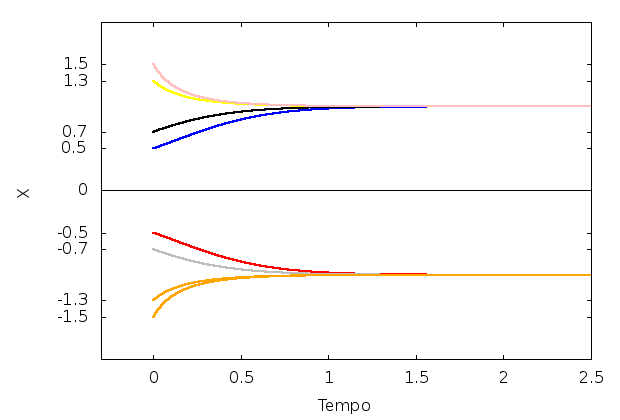
\includegraphics[width=\linewidth]{./img/analiseAssimptotica.png}
\caption{Solução analítica da EDO (\ref{ModeloDeterministicoEDO}).}
\label{fig0}
\end{minipage} \hfill
\end{figure}
Visualizamos $x(t)$ sob diversas condições iniciais, as quais são representadas pelas seguintes curvas: Cinza $x(0) = -0.5$,  verde $x(0) = -0.7$, vermelha $x(0) = -1.3$, laranja $x(0) = -1.5$, amarela $x(0) = 0.5$, azul $x(0) = 0.7$, preta $x(0) = 1.3$ e rosa $x(0) = 1.5$. Na figura (\ref{fig0}) apresentamos a dinâmica de $x_{0}$ como função do tempo de acordo com a condição inicial. Para $x(0)$ positivo, temos convergência para a solução de equilibrio assimptótico $\overline{x}_{+} = a$ e, convergência para $\overline{x}_{-} = -a$ em caso de $x(0)$ negativo. Uma característica que independe do estado inicial do sistema é seu decaimento para o regime estacionário. O parâmetro $a$, determina um tempo máximo para a meia-vida do regime dinâmico, dado como $\frac{1}{4a^{2}}$. Podemos observar que no caso de condições iniciais satisfazendo $x(0) > 0$, temos o limite assimptótico:
\begin{eqnarray}
\lim_{x \rightarrow +\infty} x(t) ,
\end{eqnarray}
e para o caso de condições iniciais satisfazendo $x(0) < 0$, temos o limite assimptótico:
\begin{eqnarray}
\lim_{x \rightarrow -\infty} x(t) .
\end{eqnarray}
Os gráficos confirmam que a vizinhança dos valores de $\overline{x}_{\pm}$ são condições de equilíbrio estável do sistema, conforme discutido no capítulo 3. Note que estamos tratando um sistema dissipativo, em que não ocorrem oscilações.

\section{Resultados EDE}
Nessa seção exibimos graficamente, a dinâmica da solução analítica da EDE (\ref{Cubo}). Assumimos o parâmetro de etiquetagem igual a uma unidade ($a = 1 $ e $ a = -1$). A solução apresentada na equação (\ref{Cubo}) toma a forma:
\begin{eqnarray}\label{eq11111222}
x_{n+1} = x_{n} - 2x_{n}(x_{n} - a)(x_{n} + a)h + \sigma N(0,1) \sqrt{h}
\end{eqnarray}
\begin{figure}[!htb]
\centering
\begin{minipage}[b]{0.9\linewidth}
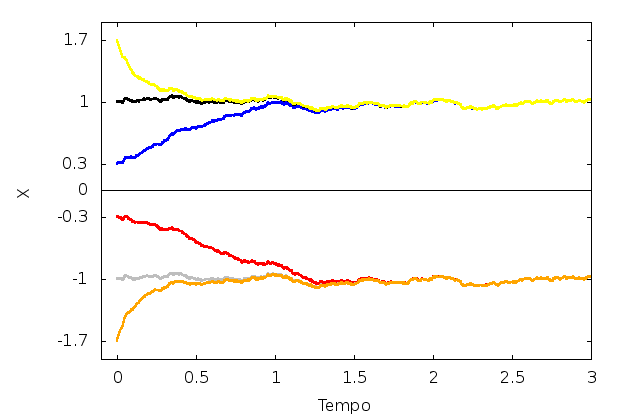
\includegraphics[width=\linewidth]{./img/analiseAssimptoticaEM.png}
\caption{Solução numérica da EDE (\ref{Cubo}).}
\label{fig0000}
\end{minipage} \hfill
\end{figure}
Visualizamos $x(t)$ sob diversas condições iniciais, as quais são representadas pelas seguintes curvas: amarela $x(0) = 1.7$, preta $x(0) = a$, azul $x(0) = 0.3$, vermelha $x(0) = -0.3$, cinza $x(0) = -a$ e laranja $x(0) = -1.7$. Uma característica que independe do estado inicial do sistema é seu decaimento para o regime estacionário. O parâmetro $a$, determina um tempo máximo para a meia-vida do regime dinâmico, dado como $\frac{1}{4a^{2}}$. Podemos observar que no caso de condições iniciais satisfazendo $x(0) > 0$, temos o limite assimptótico:
\begin{eqnarray}
\lim_{x \rightarrow +\infty} x(t) ,
\end{eqnarray}
e para o caso de condições iniciais satisfazendo $x(0) < 0$, temos o limite assimptótico:
\begin{eqnarray}
\lim_{x \rightarrow -\infty} x(t).
\end{eqnarray}

\section{Resultados EDE x EDO}
Nessa seção serão comparados os resultados da EDO com a EDE para diferentes valores de ruído.
Incluímos as trajetórias para $x(t)$ sob a condição inicial $x(0) = 0.7$. Assumindo o parâmetro de etiquetagem igual à unidade ($a=1$). Nós mostramos que valores da amplitude de ruído influenciam o comportamento do sistema em tempos assimptóticos como segue:

\begin{itemize}
\item[i)]   $\sigma = 0.1 \textrm{ , } x(t) \textrm{ \mbox{f}lutua em torno do valor de } \overline{x}_{+} = 1$;

\item[ii)]  $\sigma = 0.5\textrm{ , } x(t) \textrm{ \mbox{f}lutua em torno de } \overline{x}_{+} = 1$ 
por um certo intervalo e salta para a vizinhança de $\overline{x}_{-} = -1$ , flutuando nessa região;

\item[iii)] $\sigma = 2 \textrm{ , } x(t) \textrm{ \mbox{f}lutua em torno de } \overline{x}_{+} = 0$, desvio padrão da ordem de 1.
\end{itemize}

Agora serão exibidos os gráficos que plotamos a fim de facilitar a análise da solução da 
EDO com diferentes valores de ruído.

\begin{figure}[!htb]
\centering
\begin{minipage}[b]{0.55\linewidth}
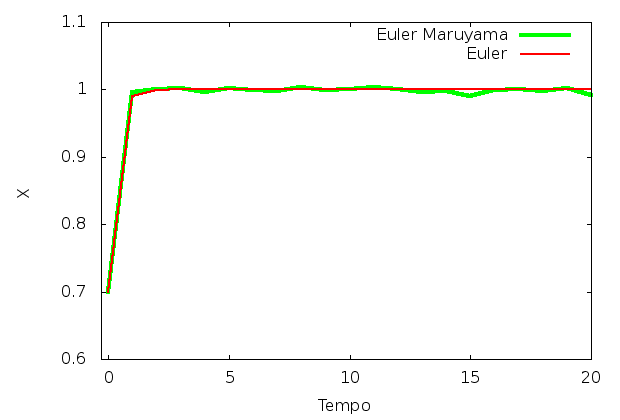
\includegraphics[width=\linewidth]{./img/Langevin_CI07_ruido001.png}
\caption{Onde $x(0) = 0.7 ; a = 1 ; \sigma = 0.01$}
\label{fig1}
\end{minipage} \hfill
\end{figure}

Na figura \ref{fig1} analisamos a dinâmica de $x$ para $\sigma = 0.01$ e condição inicial, $x(0) = 0.7$ para a 
equação ${dx} = -2x(x-a)(x+a)dt + \sigma N(0,1) \sqrt{dt}$ (\ref{Cubo}) utilizando o algorítmo de Euler-Maruyama, 
eq. $X_n = X_{n-1} + 2X_{n-1}(X_{n-1} - a)(X_{n-1} + a)h + \sigma N(0,1) \sqrt(h)$ (\ref{EM}).

Neste caso, verificamos que $x(t)$ é um processo estocástico cujos valores: $x(t_{0}, t_{1}, t_{2},...)$ para 
$t_{0} < t_{1} < t_{2}$, flutuam aleatóriamente em torno de dois valores de equilíbrio assimptótico da EDO (\ref{ModeloDeterministicoEDO}) $ \pm a$. Essa característica interessante se deve ao aumento do valor de $\sigma$." Antepenultimo da seção de resultados 4.

\begin{figure}[!htb]
\centering
\begin{minipage}[b]{0.55\linewidth}
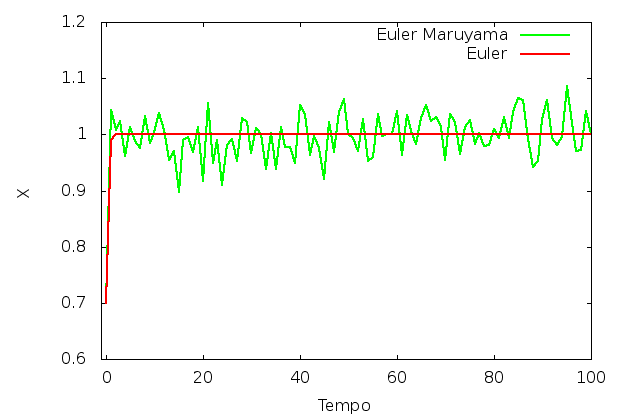
\includegraphics[width=\linewidth]{./img/Langevin_CI07_ruido01.png}
\caption{Onde $x(0) = 0.7 ; a = 1 ; \sigma = 0.1$}
\label{fig2}
\end{minipage} \hfill
\end{figure}

Na figura \ref{fig2} analisamos a dinâmica de $x$ para $\sigma = 0.1$ e condição inicial, $x(0) = 0.7$ para a 
equação ${dx} = -2x(x-a)(x+a)dt + \sigma N(0,1) \sqrt{dt}$ (\ref{Cubo}) utilizando o algorítmo de Euler-Maruyama, 
eq. $X_n = X_{n-1} + 2X_{n-1}(X_{n-1} - a)(X_{n-1} + a)h + \sigma N(0,1) \sqrt(h)$ (\ref{EM}).

Neste caso, verificamos que $x(t)$ é um processo estocástico cujos valores: $x(t_{0}, t_{1}, t_{2},...)$ para 
$t_{0} < t_{1} < t_{2}$, flutuam aleatóriamente em torno do valor assimptótico determinístico $x^{+}(+\infty) = 1$ correspondente à condição inicial assumida $x(0) = 0.7$, porém, esse valor de $\sigma$ consegue causar uma perturbação 
maior na solução.

\begin{figure}[!htb]
\centering
\begin{minipage}[b]{0.55\linewidth}
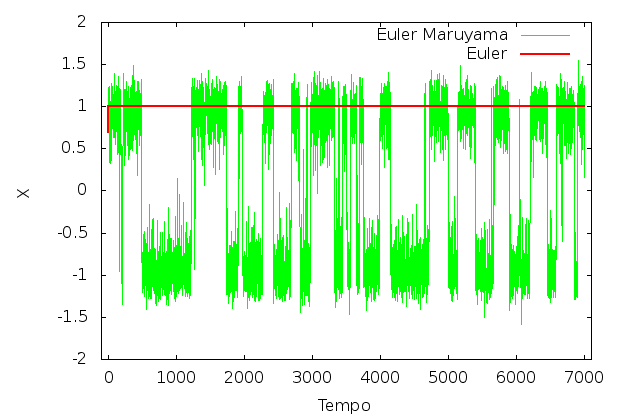
\includegraphics[width=\linewidth]{./img/Langevin_CI07_ruido05.png}
\caption{Onde $x(0) = 0.7 ; a = 1 ; \sigma = 0.5$}
\label{fig3}
\end{minipage} \hfill
\end{figure}

Na figura \ref{fig3} analisamos a dinâmica de $x$ para $\sigma = 0.5$ e condição inicial, $x(0) = 0.7$ para a eq. 
${dx} = -2x(x-a)(x+a)dt + \sigma N(0,1) \sqrt{dt}$ (\ref{Cubo}) utilizando o algorítmo de Euler-Maruyama: 
$X_n = X_{n-1} + 2X_{n-1}(X_{n-1} - a)(X_{n-1} + a)h + \sigma N(0,1) \sqrt(h)$ (\ref{EM}).

Neste caso, verificamos que $x(t)$ é um processo estocástico cujos valores: $x(t_{0}, t_{1}, t_{2},...)$ para 
$t_{0} < t_{1} < t_{2}$, flutuam aleatóriamente em torno de dois valores assimptóticos: o valor  $x^{+}(+\infty) = 1$ correspondente à condição inicial assumida $x(0) = 0.7$, e o valor $x^{-}(+\infty) = -1$, que representam os valores de a e -a, respectivamente, no caso determinístico. Essa característica interessante se deve ao aumento do valor de $\sigma$.

\begin{figure}[!htb]
\centering
\begin{minipage}[b]{0.55\linewidth}
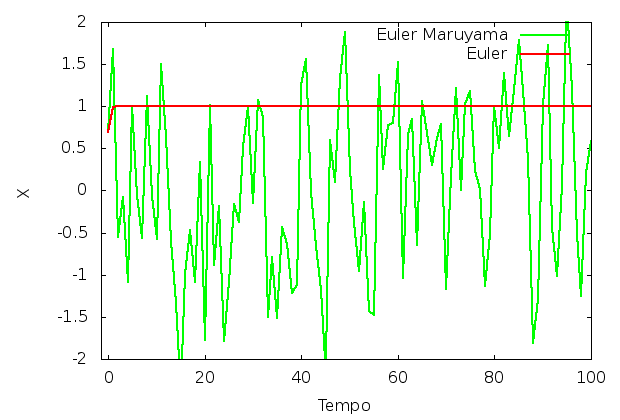
\includegraphics[width=\linewidth]{./img/Langevin_CI07_ruido2.png}
\caption{Onde $x(0) = 0.7 ; a = 1 ; \sigma = 2$}
\label{fig4}
\end{minipage} \hfill
\end{figure}

Na figura \ref{fig4} analisamos a dinâmica de ${x}$ para ${\sigma} = 2$ e condição inicial, $x(0) = 0.7$ para a eq. ${dx} = -2x(x-a)(x+a)dt + \sigma N(0,1) \sqrt{dt}$ (\ref{Cubo}) utilizando o algorítmo de Euler-Maruyama, 
eq. $X_n = X_{n-1} + 2X_{n-1}(X_{n-1} - a)(X_{n-1} + a)h + \sigma N(0,1) \sqrt(h)$ (\ref{EM}).

Neste caso, verificamos que $x(t)$ é um processo estocástico cujos valores: $x(t_{0}, t_{1}, t_{2},...)$ para 
$t_{0} < t_{1} < t_{2}$, flutuam aleatóriamente não apresentando um resultado tão interessante quanto o $\sigma = 0.5$.
%--------------------------------------------------------------------%
%-------------Término dos Resultados e Discussão---------------------%
%--------------------------------------------------------------------%


%--------------------------------------------------------------------%
%--------------------Análise dos códigos-----------------------------%
%--------------------------------------------------------------------%
\chapter{Aspectos numéricos}
Nesta seção serão analisados os algoritmos principais do nosso projeto, entre eles: solução numérica da EDO (\ref{ModeloDeterministicoEDO}), solução analítica da EDO (\ref{ModeloDeterministicoEDO}), solução numérica da EDE(\ref{Cubo}), as distribuições uniforme, Gaussiana, exponencial e por fim o movimento Browniano. Para cada um desses algoritmos será elaborado um gráfico com o tempo de execução em função da entrada exibindo o crescimento do tempo de execução da função e a quantidade de memória gasta por cada algoritmo. Vamos definir que complexidade espacial é a quantidade de memória alocada por uma função

\section{Distribuição uniforme}
O código (\ref{d_Uniforme}) apresenta uma simples chamada a função frand() definida como pré processor (por razões de eficiência) dentro de um laço. A complexidade espacial é de $O(n)$ pois a função aloca \textit{n} doubles onde \textit{n} é o numero de pontos. O tempo de execução em função da entrada pode ser visto na figura (\ref{TempExecUniforme}).
\begin{figure}[!htb]
\centering
\begin{minipage}[b]{0.45\linewidth}
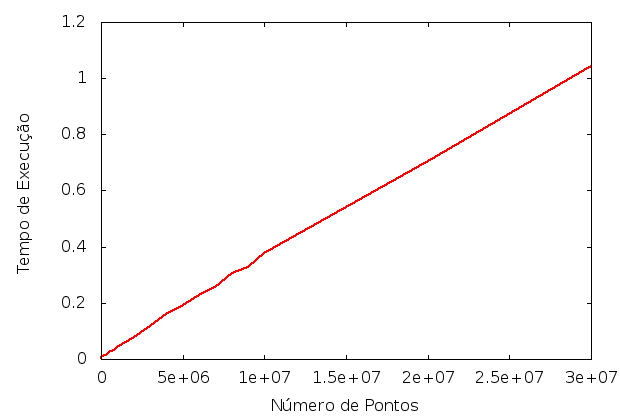
\includegraphics[width=\linewidth]{./img/AspectosNumericos/UniComplexidade.png}
\caption{Distribuição uniforme - tempo de execução}
\label{TempExecUniforme}
\end{minipage} \hfill
\end{figure}

\section{Distribuição Gaussiana}
O código (\ref{d_Gaussiana}) apresenta complexidade espacial é de O(3n) pois aloca 3 arrays de doubles 2 para distribuições uniformes e 1 para o retorno do método. O tempo de execução em função da entrada pode ser visto na figura (\ref{TempExecGau}).
\begin{figure}[!htb]
\centering
\begin{minipage}[b]{0.45\linewidth}
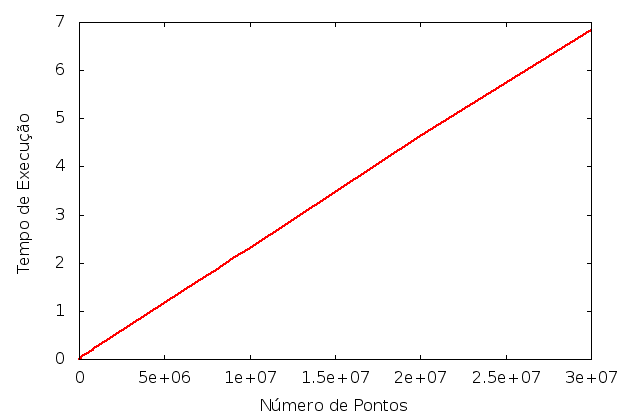
\includegraphics[width=\linewidth]{./img/AspectosNumericos/GauComplexidade.png}
\caption{Distribuição  Gaussiana- tempo de execução}
\label{TempExecGau}
\end{minipage} \hfill
\end{figure}

\section{Distribuição Exponencial}
O código (\ref{d_Exponencial}) apresenta a complexidade espacial é de O(2n) pois aloca 2 arrays de doubles 1 para distribuição uniforme e 1 para o retorno do método. O tempo de execução em função da entrada pode ser visto na figura (\ref{TempExecExp}).
\begin{figure}[!htb]
\centering
\begin{minipage}[b]{0.45\linewidth}
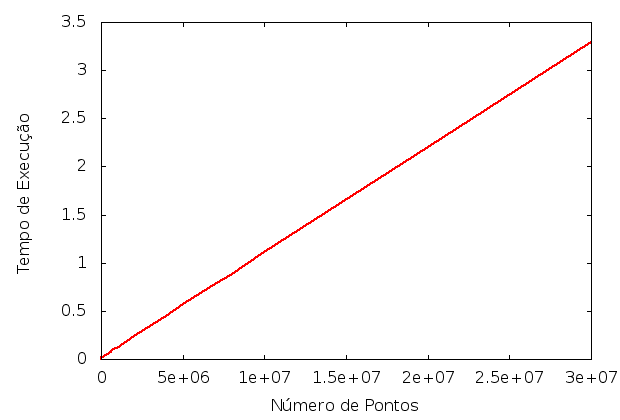
\includegraphics[width=\linewidth]{./img/AspectosNumericos/ExponencialComplexidade.png}
\caption{Distribuição exponencial - tempo de execução}
\label{TempExecExp}
\end{minipage} \hfill
\end{figure}

\section{Movimento Browniano}
O código (\ref{movimentoBrownianoFONTE}) apresenta a complexidade espacial é de $O(n)$ pois aloca um vetor de doubles para retornar o movimento discretizado. O tempo de execução em função da entrada pode ser visto na figura (\ref{movBrownianoTempExec}).
\begin{figure}[!htb]
\centering
\begin{minipage}[b]{0.45\linewidth}
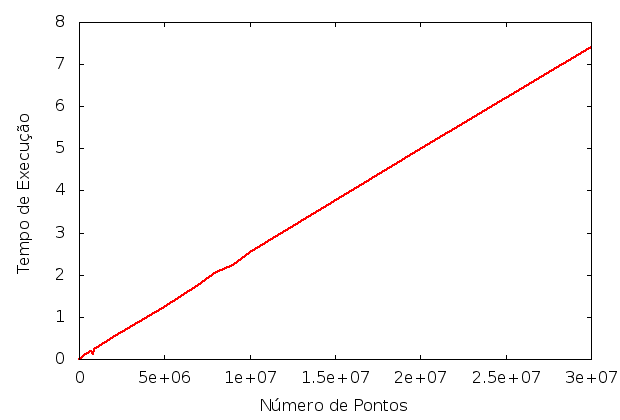
\includegraphics[width=\linewidth]{./img/AspectosNumericos/MBComplexidade.png}
\caption{Movimento Browniano- tempo de execução}
\label{movBrownianoTempExec}
\end{minipage} \hfill
\end{figure}

\section{Análise solução numérica EDO}
Ao analisar o código (\ref{EDOFONTE}) a complexidade espacial (quantidade de memória gasta) é dada como: 1 array de doubles cujo tamanho é igual ao número de pontos (n) acrescidos de dois doubles por iterada cujo escopo é o laço, logo podemos afirmar que a complexidade espacial é $O(n) * 8bytes$ (tamanho de um double em C). O tempo de execução em função da entrada pode ser visto na figura (\ref{tmpExecEuler}).
\begin{figure}[!htb]
\centering
\begin{minipage}[b]{0.45\linewidth}
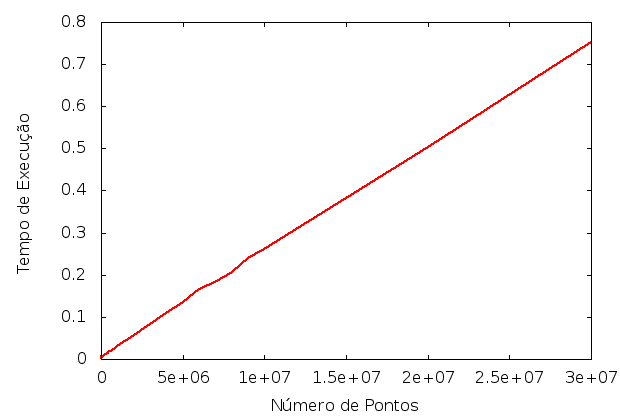
\includegraphics[width=\linewidth]{./img/AspectosNumericos/EulerComplexidade.png}
\caption{Solução númerica EDO - tempo de execução}
\label{tmpExecEuler}
\end{minipage} \hfill
\end{figure}

\section{Análise solução analítica da EDO}
Ao analisar o código (\ref{EDOFONTE}, podemos afirmar que, em termos de memória alocada a função apresenta alocação de 2 vetores de double proporcionais ao número de pontos logo a complexidade em termos de espaço é de $O(2n) * 8bytes$ (tamanho de um double em C). O tempo de execução em função da entrada pode ser visto na figura (\ref{tmpExecAnalitica}).
\begin{figure}[!htb]
\centering
\begin{minipage}[b]{0.45\linewidth}
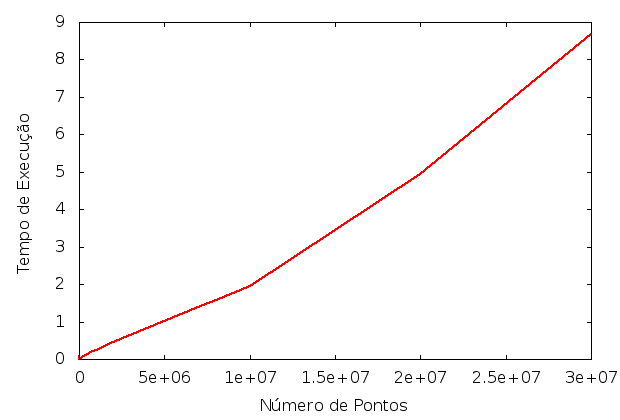
\includegraphics[width=\linewidth]{./img/AspectosNumericos/SolExacComplexidade.png}
\caption{Solução analítica EDO - tempo de execução}
\label{tmpExecAnalitica}
\end{minipage} \hfill
\end{figure}

\section{Análise solução numérica EDE Langevin}
O código (\ref{EDEFONTE}) a complexidade espacial é de O(n) dado que a função aloca n doubles para utilizar como retorno, a EDE com ruído recursivo tem a mesma complexidade porém apresenta mais multiplicações. O tempo de execução em função da entrada pode ser visto na figura (\ref{tmpExecNumericaEDE}).
\begin{figure}[!htb]
\centering
\begin{minipage}[b]{0.45\linewidth}
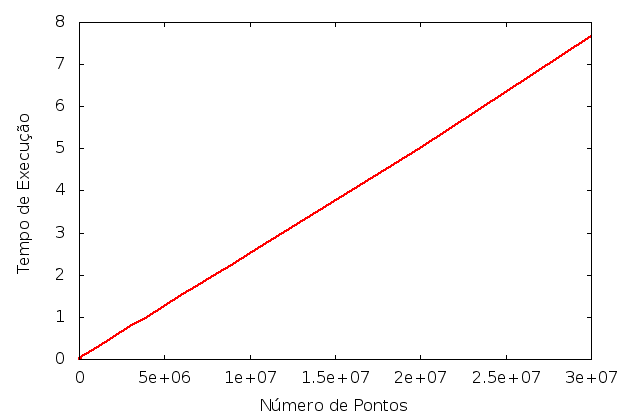
\includegraphics[width=\linewidth]{./img/AspectosNumericos/EulerMaruyamaComplexidade.png}
\caption{Solução numérica EDE - tempo de execução}
\label{tmpExecNumericaEDE}
\end{minipage} \hfill
\end{figure}



%--------------------------------------------------------------------%
%-------------Término da análise dos códigos-------------------------%
%--------------------------------------------------------------------%


%--------------------------------------------------------------------%
%---------------------------Conclusão--------------------------------%
%--------------------------------------------------------------------%
\chapter{Conclusão}
Neste trabalho de conclusão de curso, apresentamos a solução exata e numérica de uma 
EDO, equação (\ref{ModeloDeterministicoEDO}), que apresenta bi-estabilidade. A solução exata foi obtida por integração direta da EDO, enquanto 
a solução numérica foi obtida pela implementação do algoritmo de Euler em linguagem C. 
O segundo ponto importante foi estudar o efeito de perturbações estocásticas sobre esse sistema. Introduzimos uma perturbação aleatória à EDO inicial, nos moldes de Langevin, e obtivemos uma EDE, equação (\ref{triangulo}). A equação estocástica obtida foi investigada numericamente, utilizando-se o algoritmo de Euler-Maruyama. 
Mostramos que o regime estacionário do sistema aleatório guarda dependência com a intensidade do ruído. 

No caso da EDO biestável, estudamos o seu comportamento de equilíbrio, e sua dependência das 
condições iniciais do sistema. Para condições iniciais positivas, ou seja $0\le x(0) \le +\infty$, 
a solução da equação apresenta um equilibrio estável em $x = a$, para condições iniciais negativas, isto é $ 0 \ge x(0) \ge -\infty$, o sistema apresenta equilíbrio estável em $x=-a$; o sistema ainda apresenta equilíbrio instável para a soluções onde a condição inicial nula.

Ao incluirmos uma perturbação aleatória, verificamos que o comportamento assimptótico (grandes valores de tempo) do
sistema representado pela EDE depende da amplitude de ruído adicionada ao sistema.
Valores pequenos do ruído geram flutuações em torno de um limite assimptótico correspondente à
condição inicial do sistema, enquanto grandes valores da amplitude de ruído causam flutuações
em torno do limite assimptótico de equilibrio instável. É surpreendente que, para valores
intermediários da amplitude de flutuação, o comportamento assimptótico resulte em flutuações alternadas em torno
de ambos os pontos de equilíbrio estável. Pretendemos aplicar estes resultados para o estudo do
processo de determininação do destino celular.
%--------------------------------------------------------------------%
%----------------------Término da Conclusão--------------------------%
%--------------------------------------------------------------------%


%--------------------------------------------------------------------%
%----------------Término dos Capítulos da monografia-----------------%
%--------------------------------------------------------------------%



%--------------------------------------------------------------------%
%-------------------------Bibliografia-------------------------------%
%--------------------------------------------------------------------%


%\begin{thebibliography}{99}
%\bibitem{BO,00} BOYCE, William E.; DIPRIMA, Richard C.. Elementary Differential Equations and Boundary Value Problems. New York: Wiley, 2000.
%
%\bibitem{BRA,10} BRAUMANN, Carlos. \textbf{Biomatemática}. Disponível em:
%<http://www.dmat.uevora.pt/evm07/MatApoio.html>. Acesso em: 05 Mar. 2010.
%
%\bibitem{CP,11} CPROGRAMING.COM. \textbf{Debugging Segmentation Faults and Pointer Problems}. Disponível em: <http://www.cprogramming.com/debugging/segfaults.html>. Acesso em: 25 maio 2011. 
%
%\bibitem{DA,11} DAWKINS, Prof° Dr. Paul. Paul's Online Math Notes: Differential Equations - Notes. Disponível em: 
%<http://tutorial.math.lamar.edu/Classes/DE/Definitions.aspx>. Acesso em: 18 dez. 2011.
%
%\bibitem{FM,13} FERREL, James E.;MACHLEDER, Eric M. \textbf{The Biochemical Basis of an All-or-None Cell
%Fate Switch in Xenopus Oocytes} Disponível em: <http://www.sciencemag.org/content/280/5365/895.abstract>. Acesso em: 6/11/2011
%
%\bibitem{HI,01} HIGHAM, Desmond J.. \textbf{An Algoritmic Introduction to Numerical Simulation of Stochastic Differential Equations.} SIAM Rev., v. 43, n. 3, p.525-546, 01 ago. 2001.
%
%\bibitem{KL,95} KLOEDEN, Peter E.; PLATEN, Eckhard. \textbf{Numerical Solution of Stochastic Differencial Equations.} New York: Springer, 1995. 625 p
%
%\bibitem{PO} PODOLSKY, Dmitry I. On triviality of λφ4 quantum field theory in four dimensions. Disponível em: <http://arxiv.org/abs/1003.3670>. Acesso em: 18 mar. 2010.
%
%\bibitem{RY,10} RYAN, Mark. \textbf{Cálculo para Leigos.} 2. ed. Wikinnetka,illinois: Alta Books, 2010.
%
%\bibitem{SA,11} SALINAS, Silvio R.A.. \textbf{Einstein e a teoria do movimento browniano.} Rev. Bras. Ensino Fís., São Paulo, v. 27, n. 2, June 2005 .  Available from <http://www.scielo.br/scielo.php?script=sci_arttext&pid=S1806-11172005000200013&lng=en&nrm=iso>. access on 08 Mar. 2011.
%
%\bibitem{SU,10} SAUER, Timothy. \textbf{Numerical Solution of Stochastic Differencial Equations in Finance.} Disponível em: <http://math.gmu.edu/~tsauer/>. Acesso em: 8 mar. 2010.
%
%\bibitem{ST} STEWART, James. Cálculo 2. São Paulo: Thomson, 2006

%\bibliography{bib/example}


% Importa o arquivo *.bib
\bibliographystyle{apalike}
\bibliography{mestre}


%--------------------------------------------------------------------%
%--------------------Término da Bibliografia-------------------------%
%--------------------------------------------------------------------%


%--------------------------------------------------------------------%
%--------------------Código Fonte - Apendice A-----------------------%
%--------------------------------------------------------------------%
\appendix
\chapter{Código Fonte}

%\newpage

\begin{listing}[H]
\inputminted[  
               mathescape,
               linenos,
               numbersep=5pt,
               gobble=0,
               frame=lines,
               framesep=5mm]
{c}{src/GeradorPseudoAleatorio.c}
\caption{Gerador de números pseudo-aleatórios}
\label{label1}
\end{listing}


\begin{listing}[H]
\inputminted[  
               mathescape,
               linenos,
               numbersep=5pt,
               gobble=0,
               frame=lines,
               framesep=5mm]
{c}{src/AlocaMemoriaOrientadoAObjetos.c}
\caption{Alocação de memória encapsulada.}
\label{label2}
\end{listing}


\begin{listing}[H]
\inputminted[  
               mathescape,
               linenos,
               numbersep=5pt,
               gobble=0,
               frame=lines,
               framesep=5mm]
{c}{src/PlotaGraficos.c}
\caption{Funções para plotar gráficos.}
\label{label3}
\end{listing}


\begin{listing}[H]
\inputminted[  
               mathescape,
               linenos,
               numbersep=5pt,
               gobble=0,
               frame=lines,
               framesep=5mm]
{c}{src/GravaArquivos.c}
\caption{Funções para Gravar arquivos.}
\label{label4}
\end{listing}

\begin{listing}[H]
\inputminted[  
               mathescape,
               linenos,
               numbersep=5pt,
               gobble=0,
               frame=lines,
               framesep=5mm]
{c}{src/MatematicaVetorial.c}
\caption{Funções para matemática vetorial.}
\label{label41}
\end{listing}

\begin{listing}[H]
\inputminted[  
               mathescape,
               linenos,
               numbersep=5pt,
               gobble=0,
               frame=lines,
               framesep=5mm]
{c}{src/Diretorios.c}
\caption{Funções para manipular diretórios.}
\label{label5}
\end{listing}

\begin{listing}[H]
\inputminted[  
               mathescape,
               linenos,
               numbersep=5pt,
               gobble=0,
               frame=lines,
               framesep=5mm]
{c}{src/uniforme.c}
\caption{Funções para gerar ditribuição uniforme.}
\label{label6}
\end{listing}

\begin{listing}[H]
\inputminted[  
               mathescape,
               linenos,
               numbersep=5pt,
               gobble=0,
               frame=lines,
               framesep=5mm]
{c}{src/exponencial.c}
\caption{Funções para gerar ditribuição exponencial.}
\label{label7}
\end{listing}


\begin{listing}[H]
\inputminted[  
               mathescape,
               linenos,
               numbersep=5pt,
               gobble=0,
               frame=lines,
               framesep=5mm]
{c}{src/gaussiana.c}
\caption{Funções para gerar ditribuição gaussiana.}
\label{label8}
\end{listing}

\begin{listing}[H]
\inputminted[  
               mathescape,
               linenos,
               numbersep=5pt,
               gobble=0,
               frame=lines,
               framesep=5mm]
{c}{src/IncrementoInfinitesimal.c}
\caption{Funções para gerar incremento infinitesimal.}
\label{label9}
\end{listing}

\begin{listing}[H]
\inputminted[  
               mathescape,
               linenos,
               numbersep=5pt,
               gobble=0,
               frame=lines,
               framesep=5mm]
{c}{src/IncrementoInfinitesimal.c}
\caption{Funções para gerar incremento infinitesimal.}
\label{label10}
\end{listing}

\begin{listing}[H]
\inputminted[  
               mathescape,
               linenos,
               numbersep=5pt,
               gobble=0,
               frame=lines,
               framesep=5mm]
{c}{src/movimentoBrowniano.c}
\caption{Funções para gerar movimento Browniano.}
\label{label11}
\end{listing}


\begin{listing}[H]
\inputminted[  
               mathescape,
               linenos,
               numbersep=5pt,
               gobble=0,
               frame=lines,
               framesep=5mm]
{c}{src/Histograma.c}
\caption{Funções para gerar um Histograma.}
\label{label12}
\end{listing}


\begin{listing}[H]
\inputminted[  
               mathescape,
               linenos,
               numbersep=5pt,
               gobble=0,
               frame=lines,
               framesep=5mm]
{c}{src/Frequencia.c}
\caption{Funções para calcular frequência.}
\label{label13}
\end{listing}


\begin{listing}[H]
\inputminted[  
               mathescape,
               linenos,
               numbersep=5pt,
               gobble=0,
               frame=lines,
               framesep=5mm]
{c}{src/EDO.c}
\caption{Funções para calcular EDO.}
\label{label14}
\end{listing}


\begin{listing}[H]
\inputminted[  
               mathescape,
               linenos,
               numbersep=5pt,
               gobble=0,
               frame=lines,
               framesep=5mm]
{c}{src/EDE.c}
\caption{Funções para calcular EDE.}
\label{label15}
\end{listing}


\begin{listing}[H]
\inputminted[  
               mathescape,
               linenos,
               numbersep=5pt,
               gobble=0,
               frame=lines,
               framesep=5mm]
{c}{src/EDERecursivo.c}
\caption{Funções para calcular EDERecursivo.}
\label{label16}
\end{listing}



%--------------------------------------------------------------------%
%--------------Término do Código Fonte - Apendice A------------------%
%--------------------------------------------------------------------%


\end{document}
